\documentclass[fleqn]{llncs}
\usepackage[utf8]{inputenc}
\usepackage[bottom]{footmisc}
\usepackage{graphicx}
\usepackage{cite}
\usepackage{caption}
\usepackage{subcaption}
\captionsetup{compatibility=false}
%\usepackage{amsbsy}
\usepackage[fleqn]{amsmath}
\usepackage{booktabs}
\usepackage{breqn}
\usepackage{tikz}
\usetikzlibrary{arrows}
\usepackage{lipsum}
\usepackage[affil-it]{authblk}
\usepackage[english]{babel}
\interdisplaylinepenalty=2500
\pagenumbering{arabic}
\usepackage{array}
\usepackage[toc,page]{appendix}
\usepackage{bibnames}
\usepackage{tabto}
\usepackage{listings}

\title{Project 2 Clustering Report}
\author{Dong Xuanyu, Tiehang Duan, Yifu Yin}
\institute{Department of Computer Science and Engineering\\The State University of New York at Buffalo\\Buffalo, NY 14260, United States\\
\email{xuanyudo@buffalo.edu, yifuyin@buffalo.edu, tiehangd@buffalo.edu}}

\begin{document}

\maketitle

    \begin{abstract}
    This project implements clustering using three single thread and one Parallel algorithm. Single thread algorithms include k-means clustering, hierarchical agglomerative clustering with single link(min), and density based clustering. Parallel algorithm includes Map Reduce k-means clustering. Clustering is by definition, to find similar groups of data in a dataset, such that each group are similar to each other and different to others. Clustering is important in many fields. For example image processing, market research, data analysis and preprocess for other algorithms. \textbf{Python code with implementation is available on Github page: 
    \url{https://github.com/xuanyudo/Clustering-Project}.}
    \end{abstract}

\section{Model Description}
\subsection{K-Means}

K-Means clustering is an easy to implement, efficient and wildly used way to cluster data. Abstractly it is implemented in following steps:

1) Randomly initialize k centers.

2) Assign each data point to the closest center generated from previous step. Every points assigned to the same point is now a cluster.

3) For each cluster, calculate it's centroid. Move the center to the newly calculated centroid. 

4) Repeat Step 2 and Step 3 until clusters remain the same or centers remain the same.\\
The disadvantage of k-means includes sensitive to initialization, requirement of clusters count k, performs poorly under differing density, differing dataset size and irregular shape. There are ways to optimize initialization, but in this report we split data into k equal length clusters, and compute initial center from those clusters. 
    
\subsection{Hierarchical Agglomerative Clustering with Single Link(Minimal)}
Hierarchical Agglomerative Clustering is less efficient but no longer dependent on hyperparameter k. It is flexible and we are able to get any number of clusters by splitting down the hierarchy. In order to determine the structure of hierarchy, we need to determine the Inter-Cluster Distance function. Which includes min, max, average and centroid. In this project we are using min function. And abstractly it is implemented in following steps:

1). Set every single data point as cluster of singleton

2). For every clusters, find two clusters that contains closest data points, combine them together using two tree leaf nodes and set the their parent as the new cluster.

3) If there are more than two clusters left, repeat step 2.\\
Some advantage and disadvantage of Hierarchical Agglomerative Clustering is dependent on the Inter-Cluster Distance function, and in our case, it is good at finding clusters with arbitrary shapes, but it is sensitive to noises and outliers. 

\subsection{Density Based Clustering}
Density Based Clustering does not dependent on cluster number hyper-parameter k. It is insensitive to shape, size and outliers of the dataset. But it performs bad under varying density, and it is also sensitive to density hyper-parameter MinPts and eps. Abstractly it is implemented in following steps:

1). Find an undiscovered core point using MinPts. Which are points what have more or equal to MinPts points around it's radius range eps.

2). Find all core points within eps, add all discovered points within the range of eps of those points and add them into a new cluster.

3) If there are anymore undiscovered core point, repeat step 1.\\
Note that there is way to determine eps and MinPts by plotting sorted distance of every point to its kth nearest neighbor, but for this project, we are using MinPts = 3 and eps = 1.
\subsection{Map Reduce K-Mean}
TODO
\section{Model Implementation}
\subsection{Implementation of K-Means}
For the implementation of K-means, We have used K=5 for number of clusters. And we have implemented it similar to the pseudo code. For initialization, we split data into K clusters and generate centers from those. And then for every genes, We compute the closest center calculated using euclidean distance and add the gene into that cluster. To calculate centers, we add every points together by dimension and divide by cluster length, Then we repeat until calculated centroid is same as previous centroid.
\subsection{Implementation of Hierarchical Agglomerative Clustering with Single Link(Minimal)}
TODO

\subsection{Implementation of Density Based Clustering}
TODO

\subsection{Implementation of Map Reduce Clustering}
TODO
\section{Experiment Result}
For Data visualization, we are using PCA algorithm from sklearn.decomposition package. And as you see, the resulting graph includes one huge cluster and is hard to visually separate into clusters. And for performance of each algorithm, we use Jaccard's coefficient to determine.
\begin{figure}
	\centering
	\begin{subfigure}{1.0\textwidth}
		\centering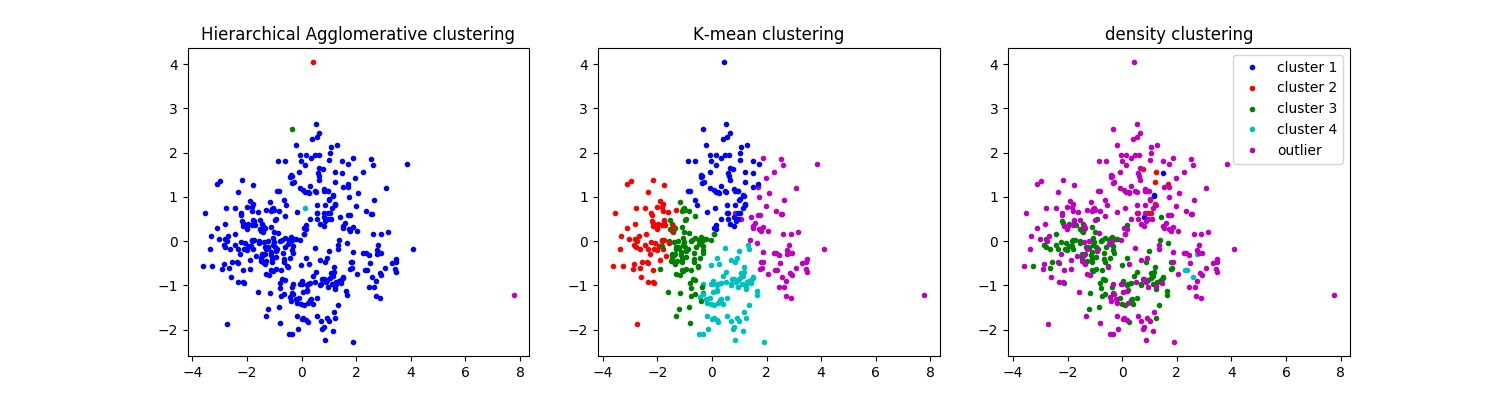
\includegraphics[width=0.7\textwidth]{hier.jpg}
		\caption{Hierarchical Agglomerative, K-Means and Density Based Algorithm}
	\end{subfigure}
	\caption{(a) Hierarchical Agglomerative clustering result visualization of cho.txt, (b) K-Means clustering result visualization of cho.txt, (c) Density Based clustering result visualization of cho.txt.}
	\label{fig2}
\end{figure}
\subsection{Result K-Means}
As you see from Fig.1, According to nature of K-means, namely poor performance toward cluster of different sizes and different density, K-means algorithm had separated the big cluster into K cluster of similar size, and split the denser cluster toward the left side into two clusters. From the graph we can conclude k-means does not perform well in this situation.

\subsection{Result Hierarchical Agglomerative Clustering with Single Link(min)}
As you see from result in Fig.1, Due to Inter-Cluster Distance function min being sensitive to outliers and noises, those points that located far away from center cluster put into it's own cluster. And the big cluster is kept as one cluster
\subsection{Result Density Based}
TODO
\subsection{Result Map Reduce Clustering}
TODO
\end{document}
